% a) MLP
\documentclass{article}
\usepackage{tikz}
\definecolor{mycolor}{HTML}{DAE8FC}
\definecolor{mycolor2}{HTML}{EDDAFC}
\begin{document}

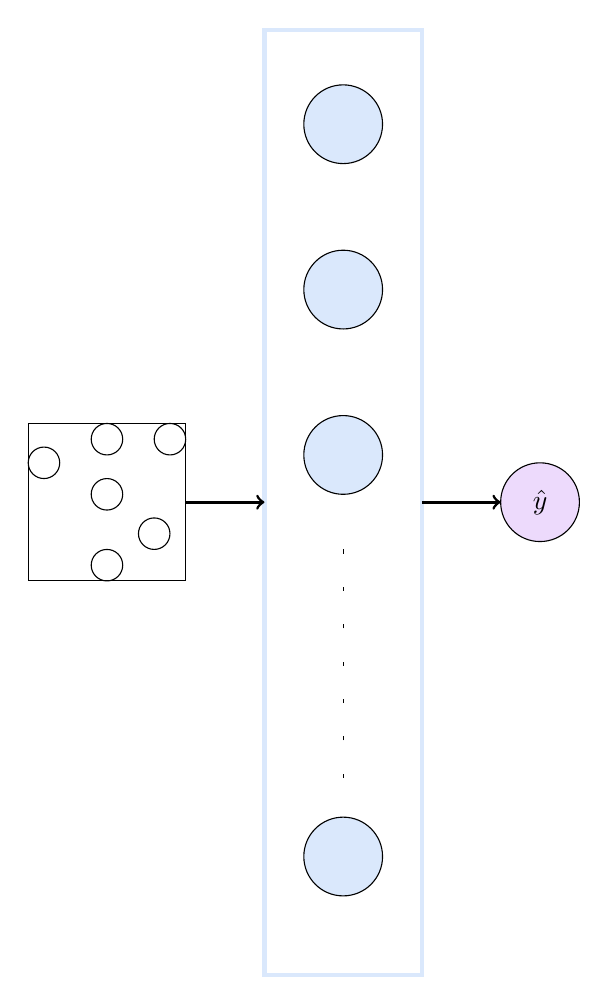
\begin{tikzpicture}

    % Middle Rectangle
    \draw[color=mycolor, line width = 1.5pt] (0, 0) rectangle (2, 12); 

    % Nodes in the hidden layer
    \foreach \i in {1,2,3} {
        \draw[fill=mycolor] (1, \i*2.1 + 4.5) circle (0.5cm); 
    }
    \draw[fill=mycolor] (1, 1.5) circle (0.5cm);

    % Dashes in rectangle between nodes
    \draw[dotted, dash pattern=on 1.5pt off 12.0pt] (1, 2.5) -- (1, 5.5);
    
    % Dataset
    % Square
    \draw (-3, 5) rectangle (-1, 7);
    % Datapoints
    \draw (-2, 5.2) circle (0.2cm);
    \draw (-2, 6.1) circle (0.2cm);
    \draw (-2, 6.8) circle (0.2cm);
    \draw (-1.2, 6.8) circle (0.2cm);
    \draw (-2.8, 6.5) circle (0.2cm);
    \draw (-1.4, 5.6) circle (0.2cm);
       
    % Arrows connecting data to hidden layers and output node
    \draw[->,  line width=1pt] (-1, 6) -- (0, 6);
    \draw[->,  line width=1pt] (2, 6) -- (3, 6);

    % output node 
    \draw[fill=mycolor2] (3.5, 6) circle (0.5cm);
    \node at (3.5, 6) {$\hat{y}$};    
    
\end{tikzpicture}
\end{document}